\chapter{SYNTH\`ESE DES CONSTATATIONS}

\section*{8.1 Statistiques globales}
\addcontentsline{toc}{section}{8.1 Statistiques globales}
La notion de non-conformit\'e de certification n'est pas applicable faute d'audit organisationnel. La synth\`ese ci-dessous porte sur le logiciel et distingue les capacit\'es valid\'ees des limites connues.

\begin{table}[H]
\centering
\caption{Indicateurs objectifs de la version finale}
\begin{tabularx}{\textwidth}{X r l}
\toprule
\rowcolor{AuditLight}Indicateur & Valeur & Source\\
\midrule
Tests backend ex\'ecut\'es & 33/33 & \evidence{manage.py test}\\
Parcours navigateur ex\'ecut\'es & 3/3 & Playwright, Chrome headless\\
Captures de rapport & 9 & sc\'enario isol\'e\\
R\^oles applicatifs & 3 & \evidence{portal.security.ROLES}\\
Outils document\'es & 4 & Nmap, Metasploit, Burp Suite, ZAP\\
Migrations applicatives & 2 & \evidence{portal/migrations}\\
Erreurs de check Django & 0 & modes d\'eveloppement et production\\
Migrations manquantes & 0 & \evidence{makemigrations --check}\\
\bottomrule
\end{tabularx}
\end{table}

\section*{8.2 R\'epartition par article / mesure}
\addcontentsline{toc}{section}{8.2 R\'epartition par article / mesure}
\begin{longtable}{p{2.4cm}p{5.4cm}p{7cm}}
\caption{Contribution technique aux mesures cibl\'ees}\\
\toprule
\rowcolor{AuditLight}Mesure & Contribution d'AuditHub & Compl\'ements organisationnels n\'ecessaires\\
\midrule\endfirsthead
\toprule Mesure & Contribution & Compl\'ements requis\\\midrule\endhead
A.8.8 & registre de constats, cible, s\'ev\'erit\'e, responsable, \`ech\'eance, correction et re-test & inventaire d'actifs complet, veille, SLA, acceptation des risques, exceptions\\
A.8.25 & RBAC, validation, sessions, tests automatis\'es, CI et guide de d\'eploiement & politique de d\'eveloppement, revues ind\'ependantes, SAST/SCA, s\'eparation des environnements\\
A.8.29 & m\'ethode, outil/version, date, preuve, empreinte et historique de re-test & plan de recette sign\'e, crit\`eres de sortie, environnement cible et validation ind\'ependante\\
\bottomrule
\end{longtable}

\begin{figure}[H]
\centering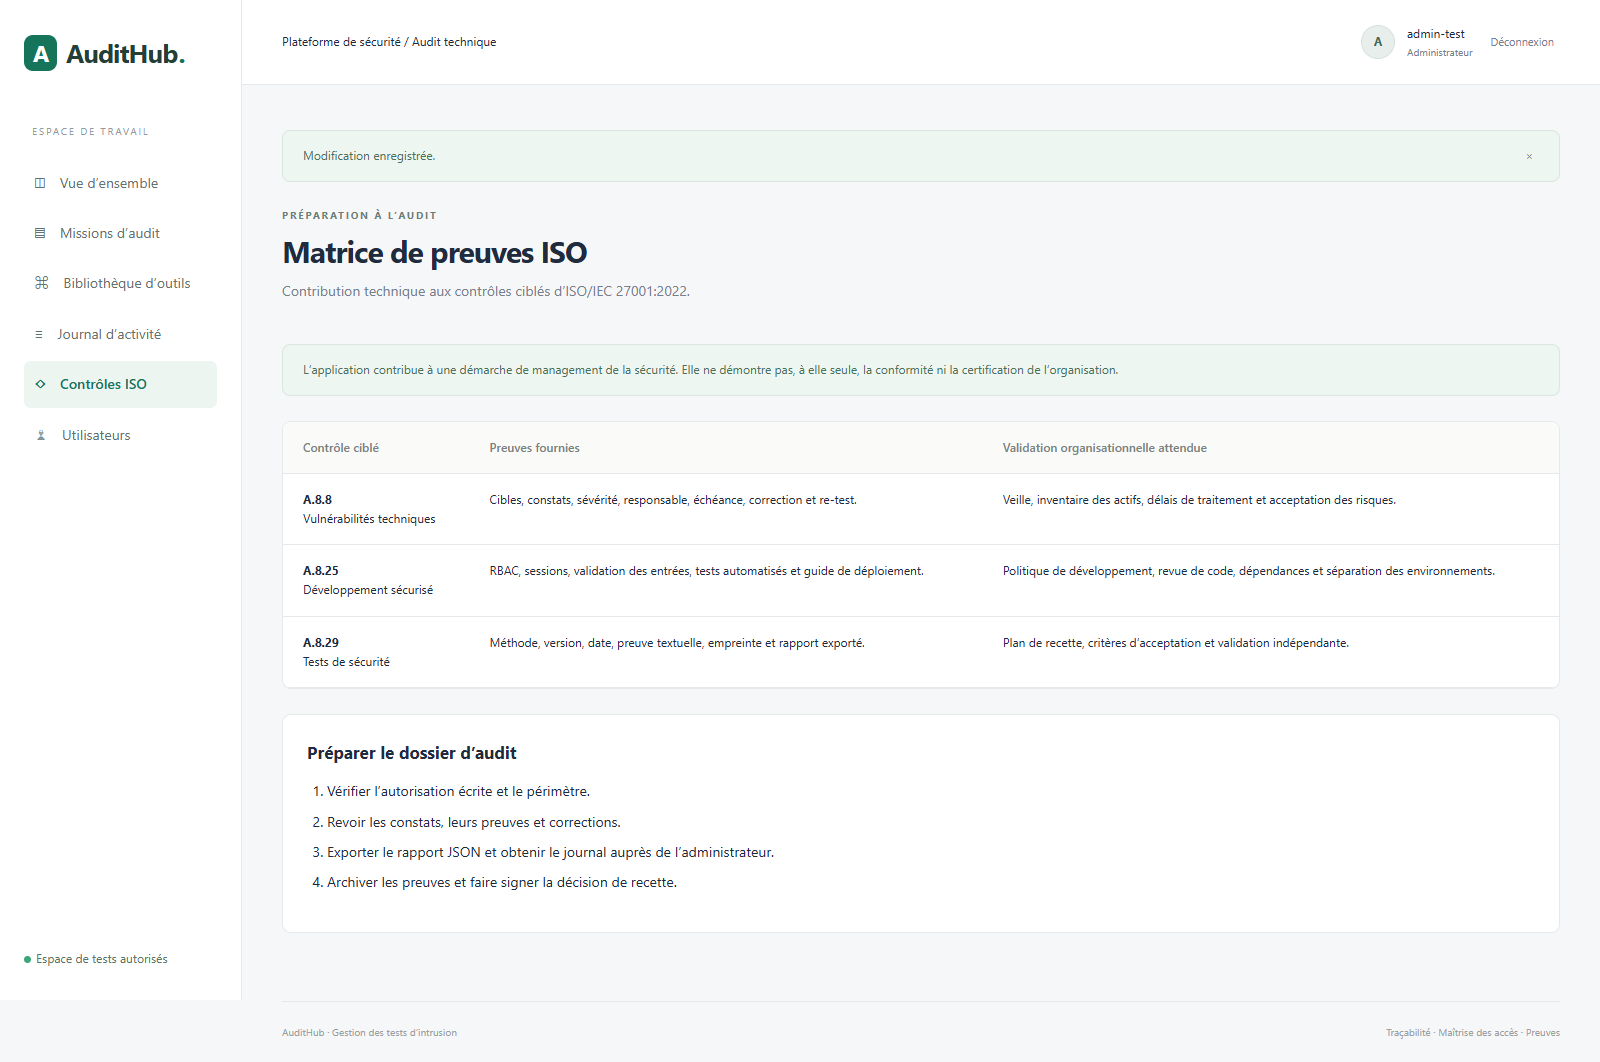
\includegraphics[width=.95\textwidth]{figures/screenshots/09-controles-iso.png}
\caption{Matrice ISO affich\'ee par l'application, explicitement pr\'esent\'ee comme contribution}
\label{fig:iso}
\end{figure}

\section*{Points forts identifi\'es}
\addcontentsline{toc}{section}{Points forts identifi\'es}
\begin{itemize}
  \item s\'eparation nette entre ex\'ecution offensive et gestion documentaire ;
  \item permissions serveur compl\'et\'ees par un cloisonnement au niveau des requ\^etes ;
  \item parcours de preuve coh\'erent, de l'autorisation \`a l'historique de correction ;
  \item gestion explicite des erreurs JSON et des erreurs de formulaires ;
  \item interface responsive sans ressource CDN et bundle reproductible via \evidence{npm ci} ;
  \item tests de s\'ecurit\'e ciblant CSRF, XSS, RBAC, p\'erim\`etre, dates, hachage et throttling ;
  \item documentation honn\^ete sur les limites et absence de revendication de certification.
\end{itemize}
